\chapter{Localizing Anomalies via Spatial-MSMA}
\label{ch:localizing}


\begin{figure}[!b]
    \centering
    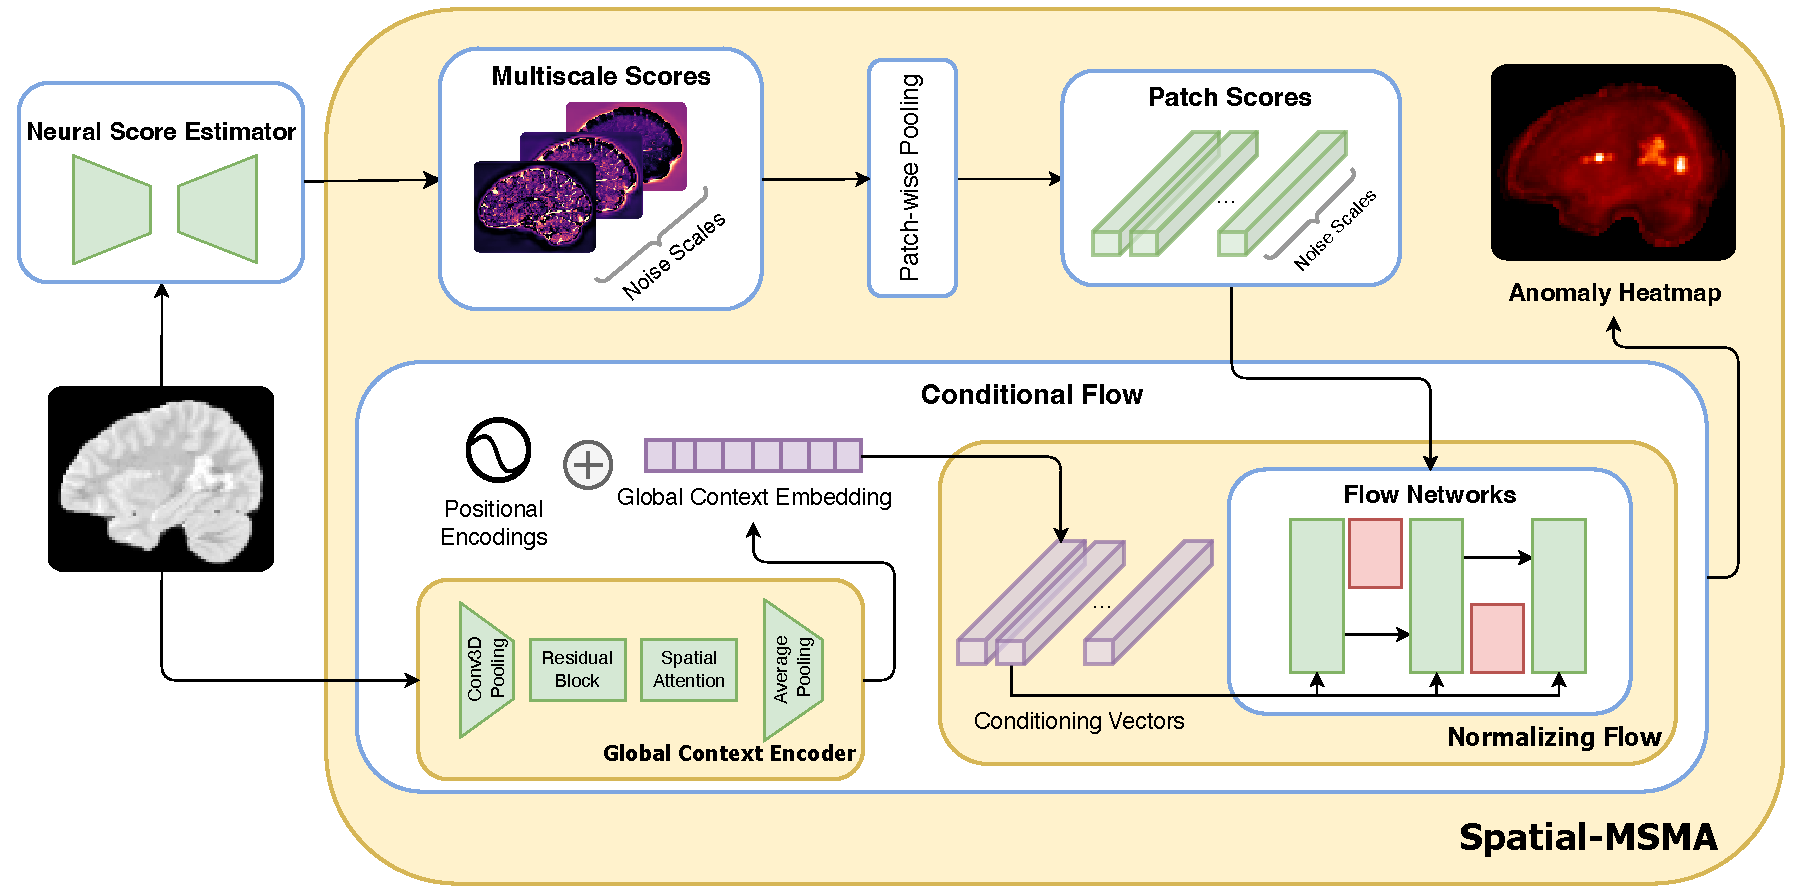
\includegraphics[width=\textwidth]{figures/spatial-msma-detailed.pdf}
    \caption{A schematic overview of Spatial-MSMA. A neural score estimator produces score tensors at multiple noise scales. The score tensors are divided into patches and processed by a conditional flow to estimate patch-wise anomaly scores. Global image features are extracted by a convolutional network and combined with positional encodings corresponding to each patch location, resulting in a conditioning vector per patch. The patch score norms and conditioning vectors are fed into a normalizing flow model with conditional coupling blocks. The result is a negative likelihood heatmap that highlights anomalous patches within the image. Spatial-MSMA thus enables precise localization of anomalies based on the patch scores and their spatial context.}
    \label{fig:spatial-overview}
\end{figure}

In the preceding chapters, we have discussed sample-wise anomaly detection. These methods operate on the full input and make binary predictions on whether a sample is anomalous. They do not, however, provide information about the input components that led to that assessment. It is often desirable to identify the specific regions within an image that are contributing to its atypicality. Such localization allows for increased model interpretability as well as directing future investigation. 

For instance, in healthcare, the ability to interpret a model's prediction empowers medical practitioners to visually corroborate the identified regions of interest. Interpretation may also pave the way for novel insights into the disease. Furthermore, localizing anomalies enables targeted diagnosis and intervention planning based on the factors contributing to the detected outlier.

Another industry where anomaly detection has critical real-world value, is manufacturing~\cite{Bergmann_2019_CVPR}. Supply chains often need to automate defect identification to reduce operational costs and time requirements. This is typically accomplished through image-based anomaly detection. As the type of defects that can emerge in production are unknown, these systems utilize unsupervised models to enable broad detection. The models are tasked to output pixel-level segmentations to help manufacturers design solutions to remediate the defects. Although many unsupervised anomaly localization methods have been proposed in recent years, it still remains an active area of research~\cite{liu2024deep}. 


This chapter will introduce Spatial-MSMA: an extended version of MSMA with localization capabilities. Note that the benefits of localization are twofold. First, it allows the possibility of pinpointing physical anomalies. For example, Spatial-MSMA is capable of highlighting brain lesions even though it was never trained with labeled data. Second, localization enables exploratory insights, gained through the interpretation of heatmaps.
% The two benefits are orthogonal with respect to one another and significantly expand the use-case for MSMA.
When taken together, these benefits significantly expand the use-case for MSMA. Related code is available at~\url{https://github.com/ahsanMah/sade/}


\section{Existing Techniques for Anomaly Localization}

\subsection*{Reconstruction based Approaches}
Reconstruction-based anomaly detectors are trained to produce typical counterparts (so-called reconstructions) of anomalous images. The methods may take some form of a deep autoencoder~\cite{dae-kascenas22a,baur2021}, trained with a reconstruction error objective such as mean squared error. At test time, the models are presumed to output an anomaly-free image, with the \textit{reconstruction error} as the metric of atypicality. A known drawback of these models is the lack of specificity in their detection. As no reconstruction is pixel-perfect (especially in terms of image intensities), the output error maps have significant false-positives~\cite{baur2021}. Another drawback of autoencoders is that as their reconstruction abilities improve, their anomaly detection capabilities decrease as the models are better at reconstructing the anomalies.

\subsection*{Generative Modeling based Approaches}

While reconstruction-based methods directly learn to reproduce typical samples, generative modeling approaches learn the underlying data distribution. These models can then use iterative sampling techniques to gradually modify the input image into a in-distribution sample. There are two main methods proposed to employ generative models for removing anomalies: \textit{imputation-based} such as ~\cite{liuUnsupervisedOutofDistributionDetection2023} or \textit{restoration-based} such as ~\cite{pmlr-v102-you19a}.

% Some methods propose to employ generative models for removing anomalies via imputation or ``restoration''~\cite{schlegl2019f,pmlr-v102-you19a}. Imputation-based approaches utilize masking strategies to mask out certain regions of the image and use the generative model to in-paint \textit{only} the masked regions. Restoration-based approaches do not use any masks and instead modify the entire image, using the original image as the starting point in the sampling procedure.

Unlike reconstruction-based approaches that attempt to recreate the entire input, imputation-based methods utilize masking strategies to selectively reconstruct certain regions of the image. Multiple passes are used to mask out different regions of the image. By focusing the network on only the unmasked regions, this approach can potentially lead to more precise anomaly localization. Restoration-based approaches, on the other hand, modify the entire image using the original image as the starting point in the sampling procedure, which can be more effective for global anomalies. The key advantage of generative modeling approaches over reconstruction-based methods is their ability to capture the probabilistic nature of the data distribution. This allows them to potentially handle a wider range of anomalies and provide more nuanced anomaly scores. However, they can be more computationally intensive and may require more complex training procedures compared to simpler reconstruction-based autoencoders.

Recently, owing to the success of score-based diffusion models, much of the research has focused on using diffusion models as the generative model (replacing GANs of yesteryear)~\citep{wyattAnoddpmAnomalyDetection2022,pinaya2022fast,liuUnsupervisedOutofDistributionDetection2023,behrendtPatchedDiffusionModels2023}. These models provide slight modifications to the diffusion sampling process, starting the generation from an input image rather than random noise. The sampling process in these generative models typically involves adding noise to the input image and iteratively denoising the sample to generate an anomaly-free counterpart of the original image. Once the cleaned sample is generated, a voxel-wise difference between the input and its anomaly-free counterpart is used as the anomaly score. This process differs from reconstruction-based methods, which directly output the reconstructed image in a single forward pass, without adding any noise to the input. The main differentiating factors between these generative modeling methods are the hyperparameters used for training and the sampling strategies used during inference, which can significantly impact their performance and computational efficiency.


% Recently, owing to the success of score-based diffusion models, much of the research has focused on using diffusion models as the generative model (replacing GANs of yesteryear)~\cite{wyattAnoddpmAnomalyDetection2022,pinaya2022fast,liuUnsupervisedOutofDistributionDetection2023,behrendtPatchedDiffusionModels2023}. All of these models provide slight modifications to the diffusion sampling process, and start the generation process from an input image rather than random noise. The sampling process starts by adding noise to the input image and iteratively denoises the sample to generate an anomaly-free counterpart of the original image. Once the cleaned sample is generated, a voxel-wise difference between the input and its anomaly-free counterpart is used as the anomaly score. The main differentiating factor between these methods are the hyperparameters used for training and the sampling strategies used during inference. 

\subsection*{Feature Embedding based Approaches}
% To circumvent the drawbacks of reconstruction errors in the image space, feature embedding based approaches compute recionstructions erroin the \textit{embedding} space.
Some methods aim to detect anomalies in a learned embedding space. The feature embeddings are computed by a neural network trained on the typical samples. At test time, it is assumed that the model will output feature embeddings that are \textit{close} to the feature embeddings of the training population if the sample is an inlier and \textit{away} otherwise. A popular method in this category is the Student-Teacher architecture anomaly detector by~\cite{bergmann2020uninformed}. In this setting, we have two models: a high parameter-count Teacher network and low parameter-count Student network. The student model is considered to be a ``weaker" version of the Teacher, and is trained using neural network distillation techniques. It is assumed that the Student model will fail to generalize to unseen datasets, producing a discrepancy between the teacher's features and that of the student. This discrepancy is used to produce an anomaly score.

\subsection*{Attribution based Approaches}
Certain anomaly detection techniques draw on the insights of interpretability research. The task is to identify features of the data that contribute to the model's output. The identified features are often assigned a score relative to their importance, as determined by the rules of the interpretation technique. Examples of such methods include SHAP~\cite{NIPS2017_7062}, Saliency Maps~\cite{Simonyan2013DeepIC}, and GradCAM~\cite{gradcam}.

SHAP (SHapley Additive exPlanations) is a game-theoretic approach to explain the output of any machine learning model. SHAP values attribute the prediction of an instance to the different features, highlighting the positive or negative impact of each feature. Saliency Maps are a visualization technique that highlight areas of an input image that most influence the output of a network. The saliency map is computed by taking the gradient of the output with respect to the input image. Areas with high gradient values correspond to regions in the input that have a significant impact on the model's prediction. GradCAM (Gradient-weighted Class Activation Mapping) is an extension of saliency maps that computes gradients with respect to feature vectors of an image rather than the image itself.

All of the mentioned attribution-based approaches aim to identify the features or input regions that contribute most to the model's predictions. This information can be used for anomaly detection, as it can localize the patches that lead a model to classify an instance as an anomaly.

\subsection*{Situating Spatial-MSMA within Existing Works}
% Maybe add a subsection, why we need Spatial MSMA, or what we expect it will do better than all of the approches discussed in 5.1. Either via a separate subsection or you can also plug the info with the respective approach subsections
Spatial-MSMA addresses key limitations of existing anomaly localization techniques. Unlike reconstruction-based approaches, it avoids the pitfall of decreasing detection capabilities as reconstruction quality improves. In contrast to generative modeling methods, Spatial-MSMA doesn't require complex sampling procedures or modifications to pretrained models. It surpasses feature embedding techniques by considering both local and global context, potentially leading to more nuanced anomaly detection. Unlike attribution-based methods that often require labeled data or focus solely on model interpretability, Spatial-MSMA offers unsupervised learning with built-in localization capabilities. By leveraging conditional likelihoods and spatial information, Spatial-MSMA is expected to provide more accurate and interpretable anomaly localization, making it particularly valuable for applications in healthcare and manufacturing where precise identification of atypical regions is crucial.

\section{Spatial-MSMA: Incorporating Spatial Information into MSMA}
The basic assumption of MSMA is that inliers will occupy distinct regions in the score-norm space. At test time, we ask the question: Does the given sample belong to the inliers? MSMA consequently estimates the likelihood of a sample belonging to the inlier region in the score-norm space. Up until this chapter we have looked at the data samples holistically, i.e. we considered the entire set of features available to us (e.g. all the pixels in an image). 

However, MSMA is also amenable for \textit{subsets} of features. For instance, we may divide an image into patches and consider the score-norms of each patch independently. Now, we can ask the question: Does this \textit{patch} belong to the inliers? As before, MSMA will output a likelihood estimate of a test patch belonging to the inliers, but this time \textit{only} considering information present at the given patch location.

It is possible to naively extend MSMA to consider patches. One can decompose the image into a regular grid, and train an independent MSMA model for each grid location. One may even reduce computational costs by running training/inference in parallel for each patch location. However, while this approach is straightforward, it leaves much room for improvement.

\subsection*{Image Patches are Not Independent of Each Other}
Namely, we can leverage \textit{spatial locality}: the notion that neighbouring image patches are highly correlated, and thus they should be assessed together for anomalies. Furthermore, even patches which are spatially apart may depend on each other. Consider an image of a face.
% Observing the patches corresponding to the left eye gives us rich information about what we may observe in regions distal to the left eye.
Observing patches of the left eye gives us rich information about what we may observe in the location of the \textit{right} eye, even if the location of the right eye is distal to the left.
One can incorporate this information into the decision making process to reason about the typicality of a queried patch. For instance, observing a brown-colored right eye is typical. However, observing a brown colored right eye \textit{given} a black-colored left eye, is atypical.

\subsection*{Modeling Conditional Likelihoods}
Following the motivation above, one can employ a conditional model where in addition to the contents of a patch, its position and surrounding context are also taken into account. As such, I posit to use a conditional likelihood model as the basis of my patch-based anomaly detector.

Concretely, the model will be conditioned on the patch position and the image features. Let $ s_p = \{s(x_p)\}_{i=1}^{L}$ be the multi-scale score tensor for a given patch $x_p$ at location $p$, belonging to the image $x$. Let $h(x)$ are the feature vectors of the image $x$ computed by a convolutional network $h$. I propose to estimate the conditional likelihood model $p(s_p | p, h(x))$. Both the flow model and the context-encoding convolutional network are trained via the Maximum Likelihood Estimation (MLE) objective. As this model will output likelihoods of score-norms for each patch conditioned on the surrounding spatial information, the model is called Spatial-MSMA.

Spatial-MSMA uses a flexible class of likelihood estimators called normalizing flows introduced in Chapter~\ref{ch:background}. The patch locations are modeled via sinusoidal positional embeddings, commonly used in Transformer models~\cite{vaswani}. In order to capture global image context, the original image is passed through a convolutional network with a large receptive field. The resulting feature embeddings are concatenated with the positional embeddings and fed into the flow model as contextual information. Recall that the feature embeddings are learned, as the convolutional network is trainable and will be updated in every backwards pass. The positional embeddings are fixed and not trained.

\section{Prototyping on 2D Images}

This section focuses on the task of segmenting anomalies in 2D images due to the availability of benchmark datasets and pretained models. A controlled experiment like this allowed me to refine the model architecture and compare Spatial-MSMA's performance to existing methodologies.

Most existing methods are trained and tested on the MvTec anomaly detection dataset~\cite{Bergmann_2019_CVPR}. This dataset focuses on industrial inspection and comprises of a set of defect-free training images and a test set of images with various kinds of manufacturing defects. The test set includes high resolution segmentation maps which allow us to validate the performance of the anomaly detection model. Note that the difficulty of this task stems from its unsupervised nature. At training time, the model will only see typical images and it cannot assume anything about the defects at the testing stage.

Similar to MSMA, Spatial-MSMA is trained in two stages. First, a score matching model is trained on the images and then the weights are frozen. Next, a likelihood model is trained on the score norms of the images. However, unlike MSMA, in Spatial-MSMA the likelihood model is trained on score norms of \textit{patches} rather than on score norms of entire images.

\subsection*{Experiment Details and Results}
To train the score-matching model, I finetuned a publicly available checkpoint~\footnote{\url{https://drive.google.com/file/d/1JInV8bPGy18QiIzZcS1iECGHCuXL6_Nz/view?usp=drive_link}} of a score-based diffusion model trained on the CIFAR-10 dataset. Next, a deep normalizing flow model is trained on the score norms for each patch, where the patch size is a fixed hyper parameter. The flow model receives the positional embeddings and the feature representations of the original image as conditioning vectors. Once the flow model is trained, we can evaluate it at every patch location in the image using a sliding-window. The resulting image is a likelihood heatmap, which is inverted to get the anomaly heatmap (negative log-likelihood).

For this experiment, the score model was trained on the \textit{Cables} class. To evaluate the anomaly detection performance, the results were compared to that of the original authors of the MvTec dataset~\cite{bergmann2020uninformed}. I compute the per-region overlap metric (PRO-AUC) introduced by the same authors, which measures the overlap between connected components in the ground truth and the anomaly map for every threshold. Even without any hyperparameter tuning, Spatial-MSMA is able to outperform the baseline by 10\% for the same patch size on the Cables class (.741 PRO-AUC vs .671 PRO-AUC).


\section{Case Study: Lesion Detection in Volumetric Brain MRIs}
Following the encouraging results on the MvTec dataset, this section will consider the more challenging task of detecting anomalies in medical images. The purpose of this case study is to reflect a real world usecase: automatic detection and segmentation of pathologies. As this is a feasibility experiment, one needs to minimize confounding factors that can be introduced due to a distributional shift between the training and testing populations. Thus, the anomalies will be simulated on a held out inlier test set, ensuring that the introduced anomalies are the \textit{primary} factor differentiating the test set from the inlier population.

\subsection*{Constructing a Healthy Population}

Our inlying, healthy population will comprise of typically developing school-age children. We chose this cohort due to the availability of public datasets within this demographic. Speicifically, we retrieved data from two studies: the Adolescent Brain Cognitive Development (ABCD) Study~\citep{Casey2018adolescent}, and the Human Connectome Project Development Study (HCP-D). Samples from these studies were preprocessed to remove any outliers. To keep the inlier cohort as nominal as possible, we used the Child Behavior Checklist (CBCL)~\cite{achenbachChildBehaviorChecklist1999} scores as our filtering mechanism. This checklist assesses the behavior and emotional competencies of children. Children with behavioral problems tend to score high on this test. The data was then split into an 80/10/10 train/validation/test split. Our processing resulted in 1320 training, 165 validation, and 165 testing samples. 

I used both T1-weighted and T2-weighted images. As the images are high-resolution 3D MRIs, they require a lot of GPU memory during training. In order to fit a batch size of 4 per GPU, the images were downsampled to a pixel spacing of 2mm isotropic. They were further cropped by the largest brain mask, computed from the training data. After some padding to make the images multiples of 2, the resulting 3D volume was of size 96x112x80. 

\subsection*{Simulating Lesions}
The anomalies were simulated using a lesion simulator tool~\cite{Filho_2019}, available as the MSLesionSimulator extension~\footnote{https://www.slicer.org/wiki/Documentation/Nightly/Modules/MSLesionSimulator} of the Slicer3D software package~\cite{fedorov3DSlicerImage2012}. The lesion load parameter was set to 20 and the rest of the hyperparameters were kept at their default values. A post processing step was performed to enhance the lesion intensity by a factor of $1.5$. The lesions were generated on the test set.


\subsection*{Training Details}
The score-norms were retrieved from a diffusion model, using a 3D convolutional UNet-like architecture. The VESDE formulation was used, with 2000 timesteps. The minimum sigma was set to 0.06, which is the average standard deviation of the image intensities. This is done so that, at minimum, the model is able to capture the intensity variation of within an image. Following the suggestion of ~\cite{song2020score}, the maximum sigma was set to 545.0 which is the 99-th percentile of the pairwise distance in the training set. This is done to allow the largest noise distribution to maximally cover the support of the data distribution i.e. $p_{\sigma_\text{max}}(x) \approx \mathcal{N}(x| 0, \sigma_\text{max}^2I)$. The model was trained for 1.5 million iterations, by which point the validation loss had started to flatten out. The batch size was doubled at roughly the half way point during training. This is a simple yet effective method proposed by~\cite{le2018dont}, to effectively anneal the learning rate without having to use a decay schedule. The authors also found that increasing the batch size also reduced the number of parameter updates required to reach the same test accuracies as strategies for decaying the learning rate.

During inference, the voxel-wise anomaly scores are first brain masked followed by thresholding. The threshold is determined for each sample by searching for the threshold that gives the lowest symmetric mean surface distance between the ground truth and the post-threshold segmentation. Searching for a threshold like this is common practice in evaluating anomaly detectors~\cite{baur_deep_2019}. The segmentations are post-processed by removing connected components of size less than 3 voxels (using a connectivity of 1). The remaining segmentation mask is dilated via a disk of radius 1 as the structuring element. Note that this inference procedure is performed for all methods tested in the experiment.

\subsection*{Baseline Methodologies}

Spatial-MSMA was compared to a selection of models that encompass a broad range of anomaly detection methodologies that have been successfully used in the medical imaging field. Namely, the baselines represent reconstruction-based, generative-based, and interpretation-based methods.
% mention why feature embedding not present..?

For the reconstruction-based baseline, I chose an autoencoder model by~\cite{aelu2023} owing to its success on volumetric brain MRIs. The model uses a ResNet-like architecture is trained using a reconstruction objective based on a Mean Squared Error (MSE). The authors also provide a publicly available implementation. This method is denoted as AE in Table~\ref{lesion_results}.

Two generative-model based approaches were also included in the comparison. First is an imputation-based approach inspired by~\cite{liuUnsupervisedOutofDistributionDetection2023} which uses a checkerboard mask to in-paint different regions of the image (denoted as Inpaint in Table~\ref{lesion_results}). This method performs multiple runs of imputation, alternating the checkerboard pattern each time and computing the average error across all runs. Second is a restoration-based approach (denoted as Restoration in Table~\ref{lesion_results}), which first adds noise to the image and then invokes the sampling procedure of the diffusion model to iteratively generate the restored counterpart. Following~\cite{wyattAnoddpmAnomalyDetection2022}, the sampling procedure was initiated from 1/4th of the original timesteps. However, unlike~\cite{wyattAnoddpmAnomalyDetection2022}, I did not use Simplex noise during training/inference as recent research has shown that it may not be necessary (and sometimes detrimental)~\cite{kascenas2023}. Note that these technique are agnostic to the diffusion framework, which allows me to use the same diffusion model that was used as the backbone of Spatial-MSMA. This keeps the comparison fair and limits confounding factors as the diffusion model was trained to convergence and is able to generate realistic looking samples.

Lastly, GradCAM was included as a representative of attribution-based approaches. Specifically, I used Guided-GradCAM~\cite{Selvaraju2016GradCAMVE} which combines saliency maps (with some modifications) and GradCAM to give superior results to vanilla GradCAM. The gradients were computed using the outputs of a non-spatial MSMA. Concretely, a GMM was trained on the whole-image score norms and the GradCAM gradients were computed using the negative likelihood estimates. This corresponds to computing voxel-wise attribution maps for an MSMA anomaly score. Thus, the method is denoted as GradCAM-MSMA in Table~\ref{lesion_results}.

\subsection*{Segmentation Metrics for Analysis}
Similar to Section~\ref{sec:cat-seg-study}, I chose mean surface distance (MSD), and the Hausdorff distance as the segmentation metrics to compare the results. These metrics compute the distance between the surfaces of the predictions and ground truth and are less biased towards over-segmentations compared to the more popular Dice score. Both distances are computed in a directed manner i.e. the distance is computed from the ground truth to the prediction. For Hausdorff distance, the 99-th percentile is used. In addition to distance metrics, component-wise metrics were also computed. Connected components were computed from the voxel-wise segmentation masks by considering an 8-connectivity-neighborhood (diagonals were included as neighbours). We assign a \textit{true positive} (TP) label to a component in the prediction which overlaps with any component in the ground-truth at any voxel location. Conversely, the absence of any overlap is used to keep a tally of the number of \textit{false positives} (FP). Table~\ref{lesion_results} reports the True Positive Rate (TPR = TP/(TP+FN)) and the Positive Predictive Value (PPV = TP/(TP+FP)). 


\begin{table*}[!ht]
\centering
\begin{tabular}{lrr|rr}
{} &        99-HD~$\downarrow$~~&      MSD~$\downarrow$~~~~~&        TPR~$\uparrow$~~~~&             PPV~$\uparrow$~~~~~\\
\midrule
AE~\citep{aelu2023} &  12.27$\pm$~0.51 &  3.63$\pm$~0.35 &  0.44$\pm$~0.02 &  0.19$\pm$~0.01 \\
Inpaint~\citep{liuUnsupervisedOutofDistributionDetection2023}       &  13.26$\pm$~0.50 &  3.71$\pm$~0.27 &  0.63$\pm$~0.02 &  0.50$\pm$~0.02 \\
Restoration~\citep{wyattAnoddpmAnomalyDetection2022}  &   8.67$\pm$~0.53 &  2.68$\pm$~0.36 &  0.68$\pm$~0.02 &  0.17$\pm$~0.01 \\
GradCAM-MSMA &  12.68$\pm$~0.54 &  3.75$\pm$~0.37 &  0.43$\pm$~0.02 &  0.16$\pm$~0.01 \\
Spatial-MSMA &  \textbf{7.05~$\pm$~0.61} &  \textbf{2.10~$\pm$~0.43} &  \textbf{0.83~$\pm$~0.01} &  \textbf{0.96~$\pm$~0.01} \\
\end{tabular}

\caption{Segmentation metrics for lesion detection. Each model was trained only on the (same) inlier samples. Right column shows distance based metrics: 99th-percentile of the Hausdorff Distance (99-HD) and Mean Surface Distance (MSD). Right column shows component-wise metrics: True Positive Rate (TPR) and Positive Predictive Value (PPV). Spatial-MSMA significantly outperforms the baseline methodologies, especially for component-wise metrics. }
\label{lesion_results}
\end{table*}

\subsection*{Results}

\begin{figure}[!tbhp]
\centering
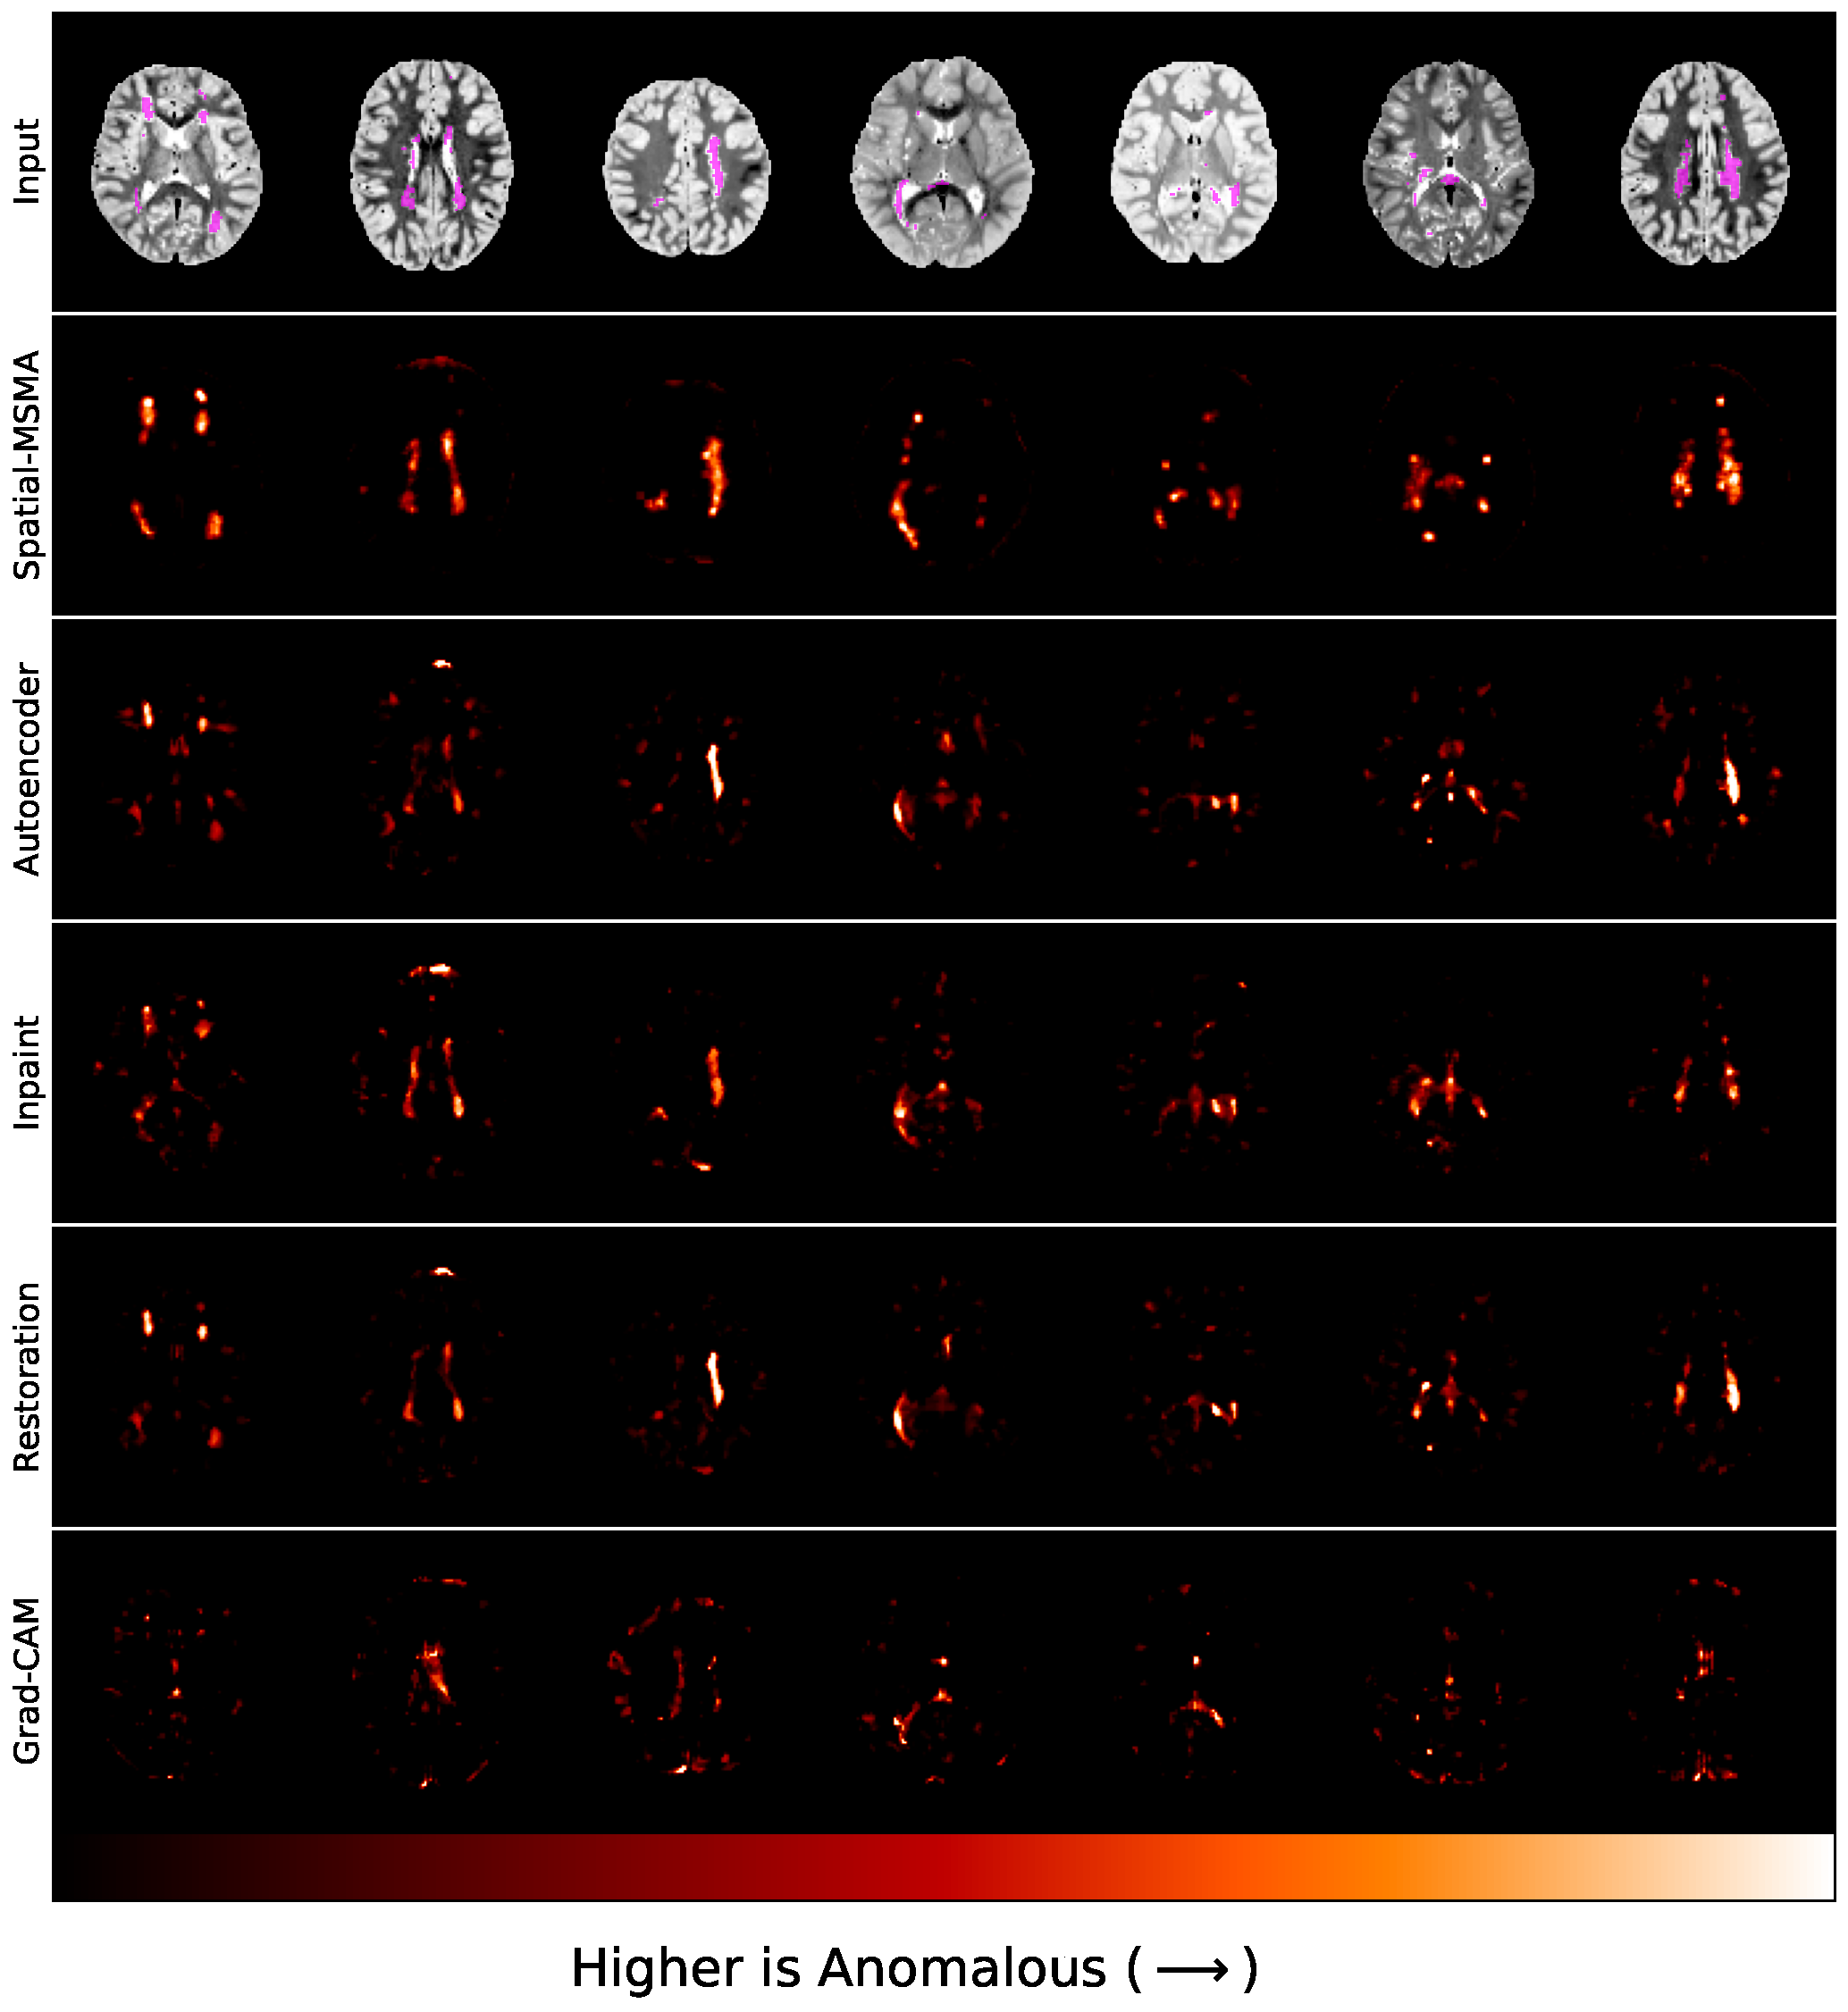
\includegraphics[width=1.01\textwidth, height=1.05\textwidth]{figures/lesion_heatmaps-l.pdf}
\caption{Qualitative comparison of anomaly heatmaps across different methods. The first row shows random axial slices of the volumetric input samples. The lesions are highlighted in magenta. Each column is a slice from random individuals. Note how Spatial-MSMA consistently detects all the lesions in the image, while other methods tend to miss smaller lesions.}
\label{fig:lesion-comp}
\end{figure}


Table~\ref{lesion_results} reports the segmentation performance of all the methods tested. Note that due to the size of the lesions, the segmentation task was difficult for all models. However, Spatial-MSMA significantly outperforms the competition. Compared to baselines, Spatial-MSMA shows the lowest distance metrics. These metrics reflect the specificity of the model's segmentation capabilities. Lower distances imply that the models segmentations have tighter boundaries around the anomalies, compared to baselines. Conversely, the component-wise metrics reflect the sensitivity of the model to anomalous regions in the image, regardless of size. Spatial-MSMA shows excellent detection capabilities, evident by the $0.83$ TPR as well as the exceptionally high PPV of $0.96$ (recall that the maximum possible PPV is 1.0). This implies that Spatial-MSMA detects few false positives, an advantageous trait in anomaly detection. We can qualitatively observe the results in Figure~\ref{fig:lesion-comp}. The plotted heatmaps are clipped at the 90th percentile for each sample i.e. the range represents the top-$10\%$ of the anomaly scores. Note that while Spatial-MSMA tends towards over-segmentation, it manages to detect most if not all the lesions. Other baselines such as Inpaint are overly biased towards larger anomalies, and often fail to detect smaller lesions.

\section{Conclusion}
This chapter introduced Spatial-MSMA: an extension to MSMA that enables localization of anomalies. The key insight is to use a conditional likelihood model to learn the distribution of patch score norms, conditioned on the patch location and surrounding context.  Spatial-MSMA demonstrated superior performance in detecting and localizing simulated lesions in volumetric brain MRIs compared to several state-of-the-art baselines. The results show that Spatial-MSMA significantly outperformed existing methods across multiple metrics, including mean surface distance, Hausdorff distance, true positive rate, and positive predictive value. While Spatial-MSMA is not expected to outperform supervised networks trained for lesion segmentation, the model's ability to detect lesions of varying sizes while maintaining a low false positive rate highlights its potential as a powerful tool for unsupervised anomaly detection in medical imaging. This chapter focused on experimentally verifying the capabilities of Spatial-MSMA using ground-truth data. The next chapter will investigate the data exploration capabilities of this approach.